%-------------------------------------------------------------------------------

% This file is part of Code_Saturne, a general-purpose CFD tool.
%
% Copyright (C) 1998-2013 EDF S.A.
%
% This program is free software; you can redistribute it and/or modify it under
% the terms of the GNU General Public License as published by the Free Software
% Foundation; either version 2 of the License, or (at your option) any later
% version.
%
% This program is distributed in the hope that it will be useful, but WITHOUT
% ANY WARRANTY; without even the implied warranty of MERCHANTABILITY or FITNESS
% FOR A PARTICULAR PURPOSE.  See the GNU General Public License for more
% details.
%
% You should have received a copy of the GNU General Public License along with
% this program; if not, write to the Free Software Foundation, Inc., 51 Franklin
% Street, Fifth Floor, Boston, MA 02110-1301, USA.
%-------------------------------------------------------------------------------

%-------------------------------------------------------------------------------
\section{Introduction}

Boundary conditions are required in at least three principal cases:
 
\begin{itemize}
\item calculation of the convection terms (first order derivative in space) at
the boundary: the calculation uses a mass flux at the boundary and requires the 
value of the convected variable at the boundary when the latter is entering 
the domain in the sense of the characteristic curves of the system;
\item calculation of the diffusion terms (second order derivative
in space):
a method to determine the value of the first order spatial derivatives 
at the boundary is then required 
 (more exactly, the fluxes that depend upon it are required,
 such as the stresses or the thermal fluxes at the wall);
\item calculation of the cell  gradients: the variable at the boundary faces
 are required (more generally, the discrete terms of the equations which depend
upon the gradient inside boundary cells are required, such as the pressure gradient or
the transpose gradient terms in the Navier-Stokes equations). 
\end{itemize}

These considerations only concern the computational variables  
(velocity, pressure, Reynolds tensor, 
scalars solution of a advection-diffusion equations \emph{etc.}). For these variables
\footnote{
The other variables 
(the physical properties for instance) have a different treatment which will 
not be detailed here (for instance, for the density, the user defines 
directly the values at the boundary. This information is then stored; one 
is referred to \fort{cs\_user\_physical\_properties} or \fort{phyvar} for more information).
},
the user has to define the boundary conditions at every boundary face.

The boundary conditions could be of Neumann type (then the flux is imposed)
or Dirichlet type (then the value of the field is prescribed), or mixed type, also 
called Robin type (then a combination of the value at the boundary and the flux
is imposed).

The code (see \fort{condli}) transforms the boundary conditions provided by the user
 into two internal formats of representation of the boundary 
 conditions. 
 
 A particular treatment is performed on walls:
 wall functions are used to model the fluid behaviour in the neighbourhood of the wall.
 Wall could be of smooth type or rough type. The modellization will be detailed in the
 coming sections.
 
A particular treatment on symmetry boundaries is also performed for vectors and tensors
whereas a symmetry boundary is equivalent to an homogeneous Neumann for scalar fields.

Two output pairs of coefficients are then computed for any variable $\varia$ for every boundary faces $\fib$:

\begin{itemize}
\item $\left( A^g_\fib , \, B^g_\fib\right)$ used by the gradient operator and by the advection operator. 
The value at the boundary face $\fib$ of the variable $\varia$ is 
then defined as:
\begin{equation}\label{eq:bndcnd:coef_g_def}
\varia_\fib \equiv A^g_\fib + B^g_\fib \varia_\centip.
\end{equation}
%
\item $\left( A^f_\ib , \, B^f_\ib\right)$ used by the diffusion operator.
The value at the boundary face $\fib$ of the diffusive flux of the variable $\varia$ 
is then defined as:
\begin{equation}\label{eq:bndcnd:coef_f_def}
D_\ib \left( K_\fib , \, \varia \right) \equiv A^f_\ib + B^f_\ib  \varia_\centip.
\end{equation}
Note that the diffusive boundary coefficients are oriented, which means that they are such that $D_\ib \left( K_\fib , \, \varia \right) $ is positive, 
this flux is gained by $\varia_\celli$.
 %
\end{itemize}
The definitions are recalled on \figurename~\ref{Base_Condli_fig_flux_condli}.

\begin{figure}[h]
\centerline{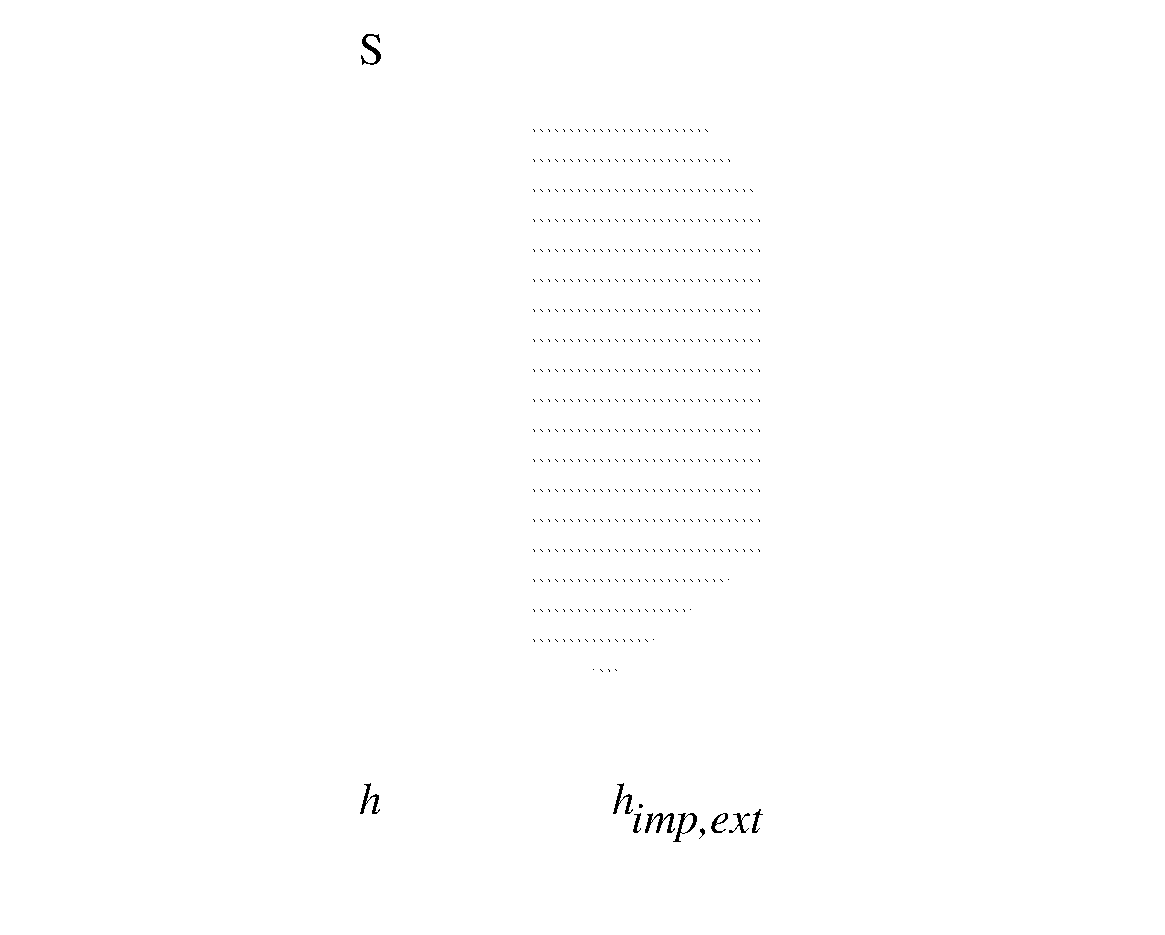
\includegraphics[height=8cm]{fluxbord}}
\caption{\label{Base_Condli_fig_flux_condli}Boundary cell.}
\end{figure}

%-------------------------------------------------------------------------------
\section{Standard user boundary conditions}

The user usually gives standard boundary conditions, which means that 
they are directly setted by the code. These standard boundary conditions are:

\begin{description}
\item[Inlet:] it corresponds to a Dirichlet boundary condition on all the transported variables 
(and should therefore be given by the user) 
and to a homogeneous Neumann on the pressure field. 

\item[Outlet:] it correspond to an homogeneous Neumann boundary condition on all the transported variables.
For the pressure field, a Dirichlet boundary condition which is expected to mimic $\displaystyle\frac{\partial^2 P}{\partial n \partial \tau}=0$ for any vector  $\vect{\tau}$ collinear to the outlet. This condition means that the pressure
profile does not vary in the direction of the outlet. Warning: if the outgoing mass-flux is negative, 
\emph{i.e.} if the outlet becomes an inlet, then the mass-flux is clipped to zero. Moreover, given
that the pressure field is defined up to a constant, it is fixed to a reference pressure $P_0$
at an arbitrary chosen outlet boundary face. 
The user can choose an other desired face where a Dirichlet on pressure is prescribed.
 
\item[Walls:] This particular treatment will be detailed in the following sections. 
For the velocity, the aim is to transform the Dirichlet boundary condition (the velocity at the wall 
is equal to the velocity of the wall) into a Neumann boundary condition where the wall shear stress
is imposed knowing the velocity of the fluid into the domain and knowing the intensity of the turbulence. 
A similar treatment using wall functions is done on every transported variable if this variable is prescribed.
The boundary condition on the pressure field is a homogeneous Neumann by default, but could
be an extrapolation of the gradient if wanted.

\item[Symmetries:] This condition corresponds to an homogeneous Neumann for the scalar fields 
(such as the pressure field or the Temperature field for instance). For vectors, such as the velocity, it corresponds
to impose a zero Dirichlet on the component normal to the boundary, and a homogeneous Neumann
on the tangential components. Thus, this condition couple the  vector components if the symmetry faces are not
aligned with the axis. The boundary condition for tensors, such as the Reynolds stresses, will be detailed in the following sections.
\end{description}

%-------------------------------------------------------------------------------
\section{Internal coding of the boundary conditions -- Discretization}

As already mentioned, the boundary conditions setted by the user for the variable $\varia$
are then translated into two pairs of coefficients $\left( A^g_\fib , \, B^g_\fib\right)$ used by the gradient operator and by the advection operator and $\left( A^f_\ib , \, B^f_\ib\right)$ used by the diffusion operator for all the boundary faces.

Let us first recall the general form of the transport equation of a variable $\varia$, which could be a scalar, 
a vector or a tensor: 
\begin{equation}\label{eq:bndcnd:gov_eqn_scalar}
\displaystyle C \rho \frac{\partial \varia}{\partial t} + C \grad \varia \cdot \left( \rho \vect{u} \right) = \dive \left(\displaystyle K \, \grad \varia \right) +ST_\varia .
\end{equation}

In the Equation (\ref{eq:bndcnd:gov_eqn_scalar})
$\rho$ is the density of the fluid, $\left( \rho \vect{u} \right)$ the convective mass flux of the variable $\varia$, $K$ its
conductivity and $S$ any additional source terms. 
Note that $K$ is the sum of molecular and turbulent diffusivity in case of RANS modelling with an eddy viscosity model. 
The dimension of $K$ for different variables is displayed in \tablename~\ref{tab:bdncnd:diffusivity}.
The value of $C$ is $1$ for all the variables except for the temperature where is value is the specific heat $C_p$.
If the variable $\varia$ is the variance of an other scalar, then its diffusivity
is deduced from the scalar itself. 

\begin{table}
{\scriptsize
\begin{center}
\begin{tabular}{||l|l|l||l|l|l||}
\hline
\multicolumn{3}{||c||}{$\varia$}&\multicolumn{3}{|c||}{$K$}\\
\hline
symbol                            & name                              & unity                    &
symbol                            & name                              & unity                  \\
\hline
$u_i$                             & velocity                          & $m.s^{-1}$                &
$\mu$ or $\mu+\mu_t$              & dynamic viscosity                 & $kg.m^{-1}.s^{-1}$     \\
$P$                               & pressure                          & $kg.m^{-1}.s^{-2}$       &
$\Delta t$                     & time step                         & $s$                      \\
$T$                               & temperature                       & $K$                        &
$\lambda$                    & thermal conductivity              & $kg.m.s^{-3}.K^{-1}$ \\
                                  &                                   &                            &
                                  &                                   & $=W.m^{-1}.K^{-1}$\\
$h$                               & enthalpy                          & $m^{2}.s^{-2}$&
$\lambda/C_p$              & thermal conductivity over specific heat  & $kg.m^{-1}.s^{-1}$     \\
                                  &                                   & $=J.kg^{-1}$&
                                  &                                   &                          \\
$\varia$                     & variable                          & unity of ($\varia$)               &
$K  $                          & conductivity or diffusivity       & $kg.m^{-1}.s^{-1}$     \\
\hline
\end{tabular}
\end{center}
}
\caption{Values and unity of $\alpha$ common cases.}\label{tab:bdncnd:diffusivity}
\end{table}

%-------------------------------------------------------------------------------
\subsection{Basic Dirichlet boundary conditions}

If the user wants to impose a basic Dirichlet condition $\varia^{imp}_\fib$ on a boundary face $\fib$,
then it is translated into:

\begin{equation}
\begin{array}{r c l}
\left\lbrace
\begin{array}{r c l}
A^g_\fib & = &\varia^{imp}_\fib , \\
B^g_\fib & = & 0,
\end{array}
\right.
 & &
\left\lbrace
\begin{array}{r c l}
A^f_\ib & = & -h_{int} \varia^{imp}_\fib, \\
B^f_\ib & = & h_{int}.
\end{array}
\right.
\end{array}
\end{equation}

The term $h_{int}$ is a internal exchange coefficient. Its value for particular variables is 
given in \tablename~\ref{tab:bndcnd:hint_phi_condli}.

\begin{remark}
Note that $\varia^{imp}_\fib$ must be specified by the user, the boundary code is $1$ (see \tablename~\ref{tab:ICODCLadm_condli}).
\end{remark}


%-------------------------------------------------------------------------------
\subsection{Neumann boundary conditions}

If the user wants to impose a Neumann condition $D^{imp}_\ib$ on a boundary face $\fib$,
then it is translated into

\begin{equation}
\begin{array}{r c l}
\left\lbrace
\begin{array}{r c l}
A^g_\fib & = & - \dfrac{D^{imp}_\ib}{h_{int}} ,\\
B^g_\fib & = & 1,
\end{array}
\right.
& &
\left\lbrace
\begin{array}{r c l}
A^f_\ib & = & D^{imp}_\ib ,\\
B^f_\ib & = & 0 .
\end{array}
\right.
\end{array}
\end{equation}

\begin{remark}
Note that  $D^{imp}_\ib$ must be specified by the user, the boundary code is $3$ (see \tablename~\ref{tab:ICODCLadm_condli}).
\end{remark}

%-------------------------------------------------------------------------------
\subsection{Advanced Dirichlet boundary conditions}
If the user wants to impose an external Dirichlet $\varia^{imp, \, ext}$ not exactly on a boundary face $\fib$ but at a small distance
related to the boundary face by an external exchange coefficient $h_{ext}$
(see \figurename~\ref{Base_Condli_fig_flux_condli}), then  the boundary condition coefficients read:

\begin{equation}
\begin{array}{r c l}
\left\lbrace
\begin{array}{r c l}
A^g_\fib & = &\dfrac{h_{ext}}{h_{int}+h_{ext}} \varia^{imp, \, ext}, \\
B^g_\fib & = & \dfrac{h_{int}}{h_{int}+h_{ext}} ,
\end{array}
\right.
& &
\left\lbrace
\begin{array}{r c l}
A^f_\ib & = & -h_{eq} \varia^{imp, \, ext} , \\
B^f_\ib & = & h_{eq},
\end{array}
\right.
\end{array}
\end{equation}
where $h_{eq} $ is defined by $h_{eq}=\dfrac{h_{int} h_{ext}}{ h_{int} + h_{ext}}$.
Note that this case reduced to the basic one if $h_{ext}$ tends to the infinity.
Also note that an outgoing flux is counted positively.

\begin{remark}
Note that both $\varia^{imp, \, ext} $ and $ h_{ext} $ must be specified by the user, the boundary code is $1$ (see \tablename~\ref{tab:ICODCLadm_condli}).
\end{remark}

%-------------------------------------------------------------------------------
\subsection{Convective outlet boundary conditions}

If the user wants to impose a convective outlet (also called radiative outlet) condition which reads:
\begin{equation}
\der{ \varia}{ t} + C \der{ \varia}{ n} = 0,
\end{equation}
where $C$ denotes the convective celerity. Then the internal coding reads:

\begin{equation}
\begin{array}{r c l}
\left\lbrace
\begin{array}{r c l}
A^g_\fib & = & \dfrac{1}{1+ CFL} \varia^n_\fib ,\\
B^g_\fib & = & \dfrac{CFL}{1+ CFL},
\end{array}
\right.
& &
\left\lbrace
\begin{array}{r c l}
A^f_\ib & = &  -  \dfrac{h_{int}}{1+ CFL} \varia^n_\fib,\\
B^f_\ib & = &  \dfrac{h_{int}}{1+ CFL},
\end{array}
\right.
\end{array}
\end{equation}
where $CFL \equiv \dfrac{C \Delta t}{\overline{\centip \centf} }$.

\begin{remark}
Note that both $C$ and $\varia^n_\fib$ must be specified by the user, the boundary code is $2$ (see \tablename~\ref{tab:ICODCLadm_condli}).
\end{remark}

\begin{table}
%{\tiny
\begin{center}
\begin{tabular}{||l|l|l||l|l||}
\hline
\multicolumn{3}{||c||}{$\varia$} & \multicolumn{2}{c||}{$h_{int}$}     \\
\hline
symbol                        & name                        & unity                    & homogeneous to                        & unity            \\
\hline
$\vect{u}$                    & velocity                    & $m.s^{-1}$               &$\dfrac{\mu+\mu_t}{ \centip \centf}$   & $kg.m^{-2}.s^{-1}$       \\
$P$                           & pressure                    & $kg.m^{-1}.s^{-2}$       & $\dfrac{\Delta t}{ \centip \centf}$   & $s.m^{-1}$                \\
$T$                           & temperature                 & $K$                      &$\dfrac{\lambda+C_p\mu_t/\sigma_t}{ \centip \centf}$  &$kg.s^{-3}.K^{-1}$\\
                              &                             &                          &                                       & $W.m^{-2}.K^{-1}$\\
$h$                           & enthalpy                    & $m^{2}.s^{-2}$           &$\dfrac{\lambda+C_p\mu_t/\sigma_t}{ \centip \centf}$ &$kg.m^{-2}.s^{-1}$\\
                              &                             & $J.kg^{-1} $             &                                                            &                                  \\
$\varia$                      & scalar                      & unity of($\varia$)       &$\dfrac{\alpha}{ \centip \centf}$      & $kg.m^{-2}.s^{-1}$       \\
\hline
\end{tabular}
\end{center}

\begin{center}
\begin{tabular}{||l|l|l||l|l||}
\hline
\multicolumn{3}{||c||}{$\varia$} & \multicolumn{2}{c||}{$D^{imp}$} \\
\hline
symbol     & name                & unity         & homogeneous to             & unity                                     \\
\hline
$\vect{u}$ & velocity            & $m.s^{-1}$         &$\left( (\mu+\mu_t)\,\gradv \vect{u} \right)\cdot \vect{n}$  & $kg.m^{-1}.s^{-2} $       \\
$p$        & pressure            & $kg.m^{-1}.s^{-2}$ &$\left( \Delta t \grad P \right) \cdot \vect{n}$             & $kg.m^{-2}.s^{-1}$                        \\
$T$        & temperature         & $K$                &$\left( (\lambda+C_p\mu_t/\sigma_t)\grad T\right) \cdot \vect{n} $ &$kg.s^{-3}$ \\
                 &                         &                                     &                                  &$W.m^{-2}$ \\       
$h$          & enthalpy           & $m^{2}.s^{-2}$          &$\left( \lambda/C_p+\mu_t/\sigma_t) \grad H \right) \cdot \vect{n}$&$kg.s^{-3}$ \\
                 &                        & $J.kg^{-1}$               &                                                                                                               & $W.m^{-2}$  \\
$\varia$   & scalar               & unity of ($\varia$)       &$K \,\grad \varia \cdot \vect{n}$              & $kg.m^{-2}.s^{-1}.$ unity of ($\varia$)       \\
\hline
\end{tabular}
\end{center}
%}
\caption{Values and unities of $h_{int}$ et $D^{imp}$  is common cases.}\label{tab:bndcnd:hint_phi_condli}
\end{table}

%-------------------------------------------------------------------------------
\subsection{Outlet boundary condition on the pressure}\label{Base_Condli_Sortie_Pression}

In this section the boundary condition on the pressure at the outlet is detailed. Some
assumptions are done to derive this boundary condition which consist of a Dirichlet
(combined with a homogeneous Neumann on the velocity) based on the pressure field
at the previous time step.
On basic configurations such as a channel or a pipe where the outlet is orthogonal 
to the flow, the shape of the pressure profile in a surface parallel to the outlet is
approximately the shape of the pressure profile at the outlet. This hypothesis 
is valid for established flows, far from any perturbation. In this configuration
one can write:

\begin{equation*}
\displaystyle\frac{\partial^2 P}{\partial n \partial \tau } = 0,
\end{equation*}
where $\vect{n}$ is the outward normal vector and  $\vect{\tau}$ is any 
vector in the boundary face.

Then remark that the value at the boundary face $\fib$ is linked
to the pressure value in $\centip$ by the relationship:
\begin{equation*}
P_\fib = P_{\centip} +  \grad_\celli P \cdot \vect{\centip\centf}.
\end{equation*}
If moreover we assume that the pressure gradient in the normal direction
is uniform, and that all the $\centip$ related to the outlet faces are on 
a single plane parallel to the outlet, then the value of $ \grad_\celli P \cdot \vect{\centip\centf} $
is constant for all the faces and denoted $R$. 

Furthermore, the pressure is defined up to a constant, so the code
chooses to fix the pressure at $P_0$ to a given outlet boundary face 
$\fib^{imp}$. Therefore the pressure field is shifted  by the constant
$R_0=P_0- P_\fib^{imp} = P_0 - \left( P_{\centip}^{imp}+R \right)$.

All that together gives
\begin{equation}\label{Base_Condli_eq_psortie_condli}
\begin{array}{rcl}
P_\fib 
   &=& P_{\centip}+R+R_0,\\
   &=& P_{\centip}+R+P_0- \left( P_{\centip}^{imp}+R \right),\\
   &=&P_{\centip} +\underbrace{P_0-P_{\centip}^{imp}}_{\text{constant denoted by $\widetilde{R}$}} ,\\
   &=&P_{\centip} + \widetilde{R}.
\end{array}
\end{equation}

To conclude, the outlet boundary condition on the pressure is a Dirichlet based on 
the value in $\centip$ (at the previous time step) and shifted to imposed
the value $P_0$ at a given face $\fib$.

%-------------------------------------------------------------------------------
\subsubsection{Checking step}

 Before computing the pairs of boundary condition coefficients, a step of checking is performed. Basically, 
the code checks that the user has given a boundary condition to all boundary faces, and that 
setting between all the variables is compatible (see \tablename~\ref{tab:ICODCLadm_condli}).



\begin{table}
%{\tiny
\begin{center}
\begin{tabular}{||c|c||p{0,6cm}|p{0,6cm}|p{0,6cm}|p{0,6cm}|p{0,6cm}|p{0,6cm}|p{0,6cm}||}
\hline
\multicolumn{2}{||c||}{Variable}
        &\multicolumn{7}{c||}{Admissible Values}\\
\hline
Velocity                                & $\vect{u}$                                                                         &  1& 2& 3& 4& 5& 6& 9 \\
Pressure                                & $P$                                                                                   &  1& 2& 3&  &  & & \\
Scalar turbulent variables     & $k$, $\varepsilon$, $\varphi$, $\bar{f}$, $\omega$        &  1& 2& 3&  & 5& 6& \\
Reynolds stresses                & $R_{ij}$                                                                              &  1& 2& 3& 4& 5& 6& \\
$\varia$ (except variances)  &  $\varia$                                                                           &  1& 2& 3&  & 5& 6& \\
Variance of a variable $\varia$ &                                                                                      &  1& 2& 3&  &  & & \\
\hline
\end{tabular}
\end{center}
%}
\caption{Admissible values of boundary conditions for all variables.}\label{tab:ICODCLadm_condli}
\end{table}
